\documentclass[12pt,titlepage]{article}
\usepackage[margin=1.25in]{geometry}
\usepackage{graphicx,amsmath,blindtext,enumitem}

%% Variables definition
\newcommand{\vSubject}{Database}
\newcommand{\vSubtitle}{ER Diagram}
\newcommand{\vName}{Dicha Zelianivan Arkana}
\newcommand{\vNIM}{2241720002}
\newcommand{\vClass}{1i}
\newcommand{\vDepartment}{Information Technology}
\newcommand{\vStudyProgram}{D4 Informatics Engineering}

%% [START] Tikz related stuff
\usepackage{tikz}
\usetikzlibrary{svg.path,calc,shapes.geometric,shapes.misc}
\tikzstyle{terminator} = [rectangle, draw, text centered, rounded corners = 1em, minimum height=2em]
\tikzstyle{preparation} = [chamfered rectangle, chamfered rectangle sep=0.75em, draw, text centered, minimum height = 2em]
\tikzstyle{process} = [rectangle, draw, text centered, minimum height=2em]
\tikzstyle{decision} = [diamond, aspect=2, draw, text centered, minimum height=2em]
\tikzstyle{data}=[trapezium, draw, text centered, trapezium left angle=60, trapezium right angle=120, minimum height=2em]
\tikzstyle{connector} = [line width=0.25mm,->]
%% [END] Tikz related stuff

%% [START] Fancy header related stuff
\usepackage{fancyhdr}
\pagestyle{fancy}
\setlength{\headheight}{15pt} % compensate fancyhdr style
\fancyhead{}
\fancyfoot{}
\fancyfoot[L]{\thepage}
\fancyfoot[R]{\textit{\vSubject - \vSubtitle}}
\renewcommand{\footrulewidth}{0.4pt}% default is 0pt, overline for footer
%% [END] Fancy header related stuff

%% [START] Custom tabular command related stuff
\usepackage{tabularx}
\newcommand{\details}[2]{
    #1 & #2  \\
}
%% [END] Custom tabular command related stuff

%% [START] Figure related stuff
\newcommand{\image}[3][1]{
    \begin{figure}[h]
        \centering
        \includegraphics[#1]{#2}
        \caption{#3}
        \label{#3}
    \end{figure}
}
%% [END] Figure related stuff

\begin{document}
\begin{titlepage}
    \centering
    \vfill
    {\bfseries\LARGE
        \vSubject\\
        \vskip0.25cm
        \vSubtitle
    }
    \vfill
    
\includegraphics[width=6cm]{images/polinema-logo.png}
    \vfill
    {
        \textbf{Name}\\
        \vName\\
        \vskip0.5cm
        \textbf{NIM}\\
        \vNIM\\
        \vskip0.5cm
        \textbf{Class}\\
        \vClass\\
        \vskip0.5cm
        \textbf{Department}\\
        \vDepartment\\
        \vskip0.5cm
        \textbf{Study Program}\\
        \vStudyProgram
    }
\end{titlepage}

\section{Learning Task}
In a library, a book title may have many copies. A copy of the book can be borrowed by a borrower.
A borrower may borrow many books. The same book copy may be borrowed by many borrowers.
The library wishes to store information about authors of books also. An authors may
have authored many books; whereas, a book may have many authors. A book title is identified
by a BookID and has Title, Copyright, and Publisher. A copy of a book is provided a CopyID
which is unique to all copies of books. The name of authors are of interset to the library and is
given an AuthorID

\begin{enumerate}[label=\Alph*.]
    \item {
        Draw the ER diagram of the case presented above!

        \begin{figure}[h]
            \centering
            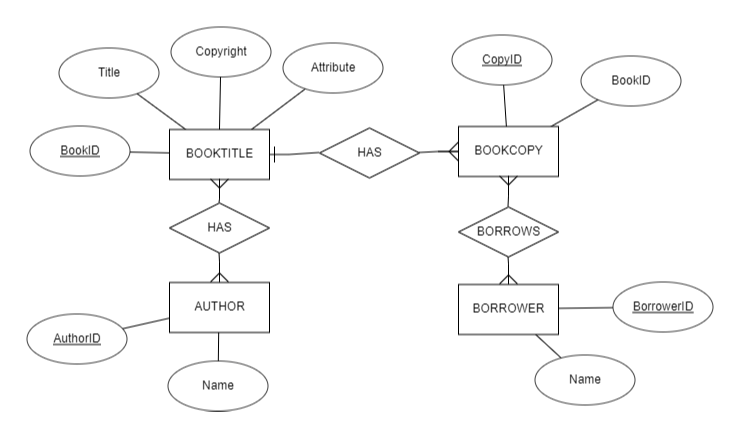
\includegraphics[width=\textwidth]{./images/erd.png}
            \caption{The Entity Relationship Diagram for the above case study}
        \end{figure}
    }
    \item {
        What relationship exists between BOOKTITLE and BOOKCOPY if there is?

        The relationship between BOOKTITLE and BOOKCOPY is 1-n or one to many.
        This is due to the fact that each BOOKTITLE can have many copies but not the other way around.
    }
    \item {
        What relationship exists between BOOKTITLE and BORROWER if there is?

        The relationship between BOOKTITLE and BORROWER is n-m or many to many.
        This is because a BOOKTITLE can be borrowed by multiple BORROWER but multiple
        BORROWER can also borrow the same BOOKTITLE.
    }
    \item {
        How many relationships or associations exist in the ER Model for the given problem?

        There are 3 relations on this case study, namely:
        \begin{itemize}
            \item Relation between BOOKTITLE and BOOKCOPY which is 1-n or one to many
            \item Relation between AUTHOR and BOOKTITLE which is n-m or many to many
            \item Relation between BORROWER and BOOKCOPY which is n-m or many to many
        \end{itemize}
    }
    \item {
        What will be the attributes of the BOOKCOPY table including the primary keys and foreign keys?

        The BOOKCOPY table will have the \texttt{CopyID} as its primary key and \texttt{BookID} as its foreign key which is used
        to connect itself to the BOOKTITLE table.
    }
    \item {
        What foreign key will be set for the BOOKTITLE and BOOKCOPY relationship?

        Since the relationship for BOOKTITLE and BOOKCOPY is many to many, there needs to be a pivot table.
        The pivot table will have the \texttt{BookID} and \texttt{CopyID} as its foreign key which refers to
        both table primary key.
    }
\end{enumerate}

\end{document}

